\documentclass[a4paper]{scrartcl}

%% Language and font encodings
\usepackage[english]{babel}
\usepackage[utf8x]{inputenc}
\usepackage[T1]{fontenc}
\usepackage{courier} 

%% Sets page size and margins
\usepackage[a4paper,top=3cm,bottom=2cm,left=3cm,right=3cm,marginparwidth=1.75cm]{geometry}

%% Useful packages
\usepackage{amsmath}
\usepackage{graphicx}
\usepackage[colorinlistoftodos]{todonotes}
\usepackage[colorlinks=true, allcolors=black]{hyperref}
\usepackage{float}
\usepackage{subfigure}
\usepackage{listings} 
\usepackage[framed,numbered,autolinebreaks,useliterate]{mcode}


\title{IN4320 Machine Learning Exercise 1 Report}
\subtitle{Exercise Regularizations \& Sparsity}
\author{ % listed by the student number in the ascending 
		Lu Liu (4621832)		
		}

\begin{document}
\maketitle
%\tableofcontents

%\clearpage
\section{Some Optima \& Some Geometry}
\label{ch:some}

\subsection{ Question 1}
The loss function L used in this assignment is:
$$L(m_-, m_+):=\sum_i^N ||x_i - m_{y_i}||^2 + \lambda||m_- - m_+||_1$$
with $\lambda$ the regularization parameter, $N$ the number of samples in the training set, and $||\cdot||_1$ the $L_1$-norm.

\subsubsection{a}
In this part, the loss function in one dimension is drawn as a function of $m_+$ for for $\lambda \in \{0,2,4,6\}$. 

\begin{figure}[h!]
\centering
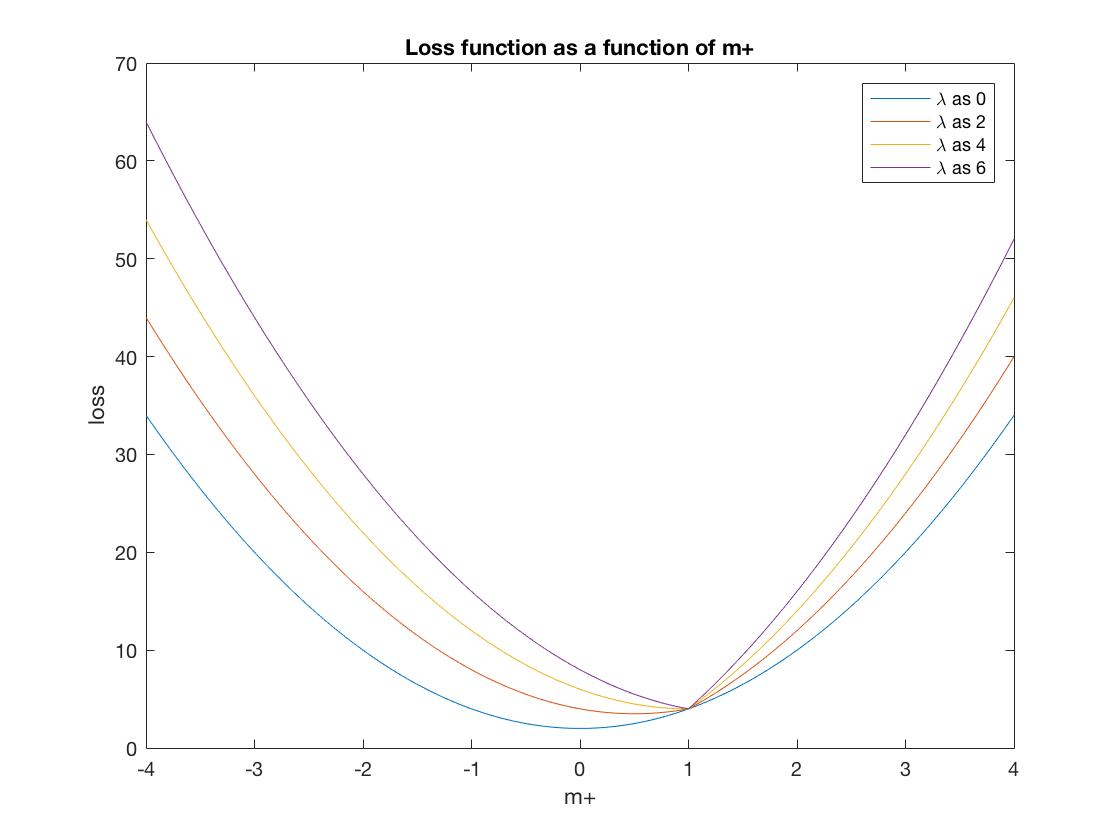
\includegraphics[width=9cm]{q1a.jpg}
\caption{Loss Function as a function of $m_+$ for for $\lambda \in \{0,2,4,6\}$}
\label{fig:q1a}
\end{figure}

\subsubsection{b}
In this part, for every of the four functions, the minimizer and their minimum values are derived as well as the point where the derivative equals 0.
Here I use MATLAB to find the points.
Since with different $\lambda$ the MATLAB code for drawing figure and finding the point with derivative as 0 is the same, here only the code for $\lambda$ as 0 is shown in Appendix \ref{app: a}.


And the answer I obtained is:
\begin{table}[!h]
\centering
\caption{Results for Question 1(b)}
\label{tab: 1core}
\begin{tabular}{|c|c c|c c|}
\hline
$\lambda$ & minimizer & minimum values & the point with derivative as 0 & its value \\
\hline
0 & 0 & 2 & 0.0100 & 2.002 \\ 
2 & 0.5 & 3.5 & 0.5100 & 3.5002 \\
4 & 1 & 4 & 1 & 4 \\
6 & 1 & 4 & 1 & 4 \\
\hline
\end{tabular}
\end{table}

When searching for the point with derivative as 0, I try to find the point with the minimum absolute value of derivative. 
Thus the points with derivative as 0.02 are found here, which is almost the same point.

\subsection{Question 2}
\subsubsection{a}
\label{subsubsection: 2.a}
In this loss function, the norm is 1. 
Thus the shape of $\lambda||m_- - m_+||_1$ is shown in Figure \ref{fig:norm}. 
It is the square placed on the origin. 
In Figure \ref{fig:norm}, the ellipses mean the contour for the first part of loss function $L$, which is $\sum_i^N ||x_i - m_{y_i}||^2$.
The intersection of them is the minimum point expected. 
If $\lambda$ is very small, there might be no intersection. Thus the mean values obtained at that time is not the optimized.
With the increase of $\lambda$, the radius of the square increases.
The intersection appears and maintains even $\lambda$ is very large. Thus the mean values obtained maintain the same with the increase of $\lambda$, which is result expected.

\subsubsection{b}
From the format of the general function $L$, it can be seen that the loss is convex. 
Thus there is only one minimum point in $L$. 
With two variables $m_-$ and $m_+$, a 3D figure can be drawn for $L$ as well as the contour lines for $L$. 
To make the figure elegant, the data given in  Section \ref{subsubsec:2.c} is used. 
The contour lines are shown in Figure \ref{fig:q2b}, and the 3D figure is shown in Figure \ref{fig:q2c}.

\begin{figure}[!h]
\begin{minipage}[t]{0.33\linewidth}
\centering
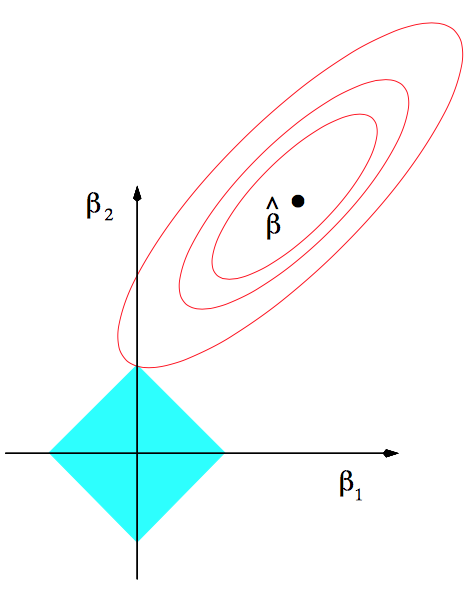
\includegraphics[width=2.2in]{norm.png}
\caption{The “classic” illustration comparing lasso and ridge constraints. From Chapter 3 of Hastie et al.(2009)}
\label{fig:norm}
\end{minipage}%
\begin{minipage}[t]{0.33\linewidth}
\centering
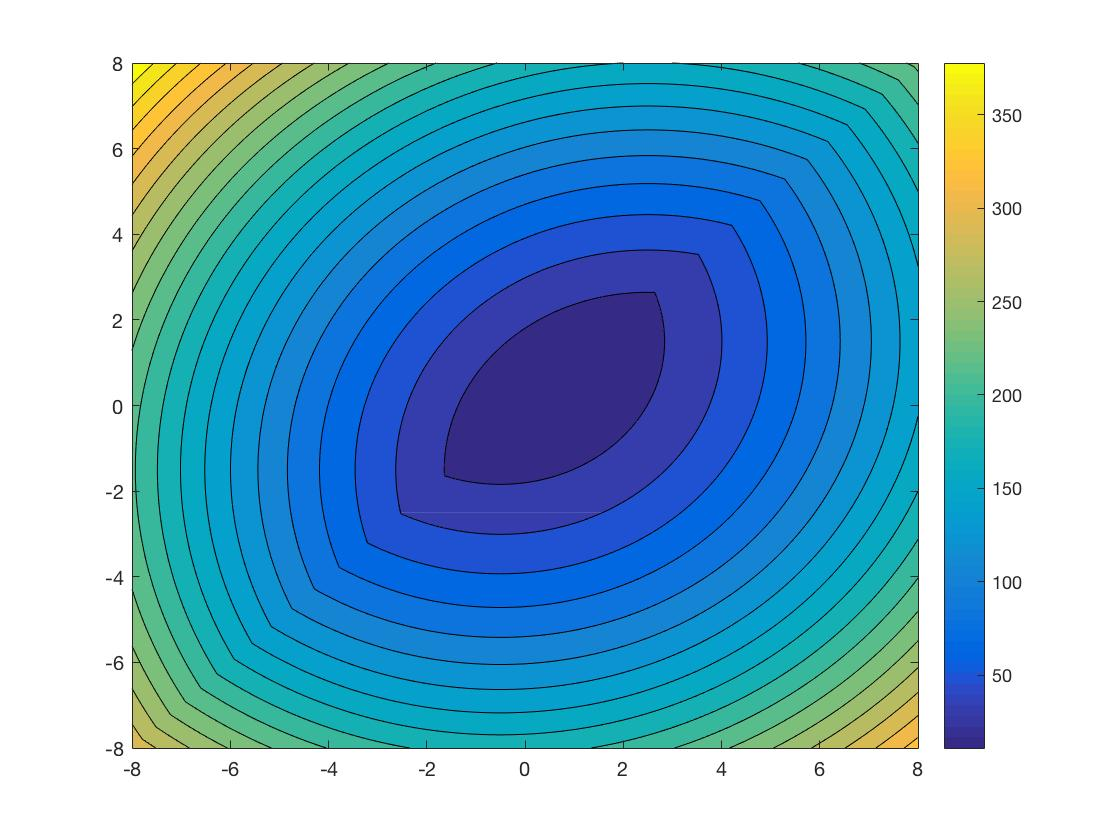
\includegraphics[width=2.2in]{q2b.jpg}
\caption{The contour lines for the general function L}
\label{fig:q2b}
\end{minipage}%
\begin{minipage}[t]{0.33\linewidth}
\centering
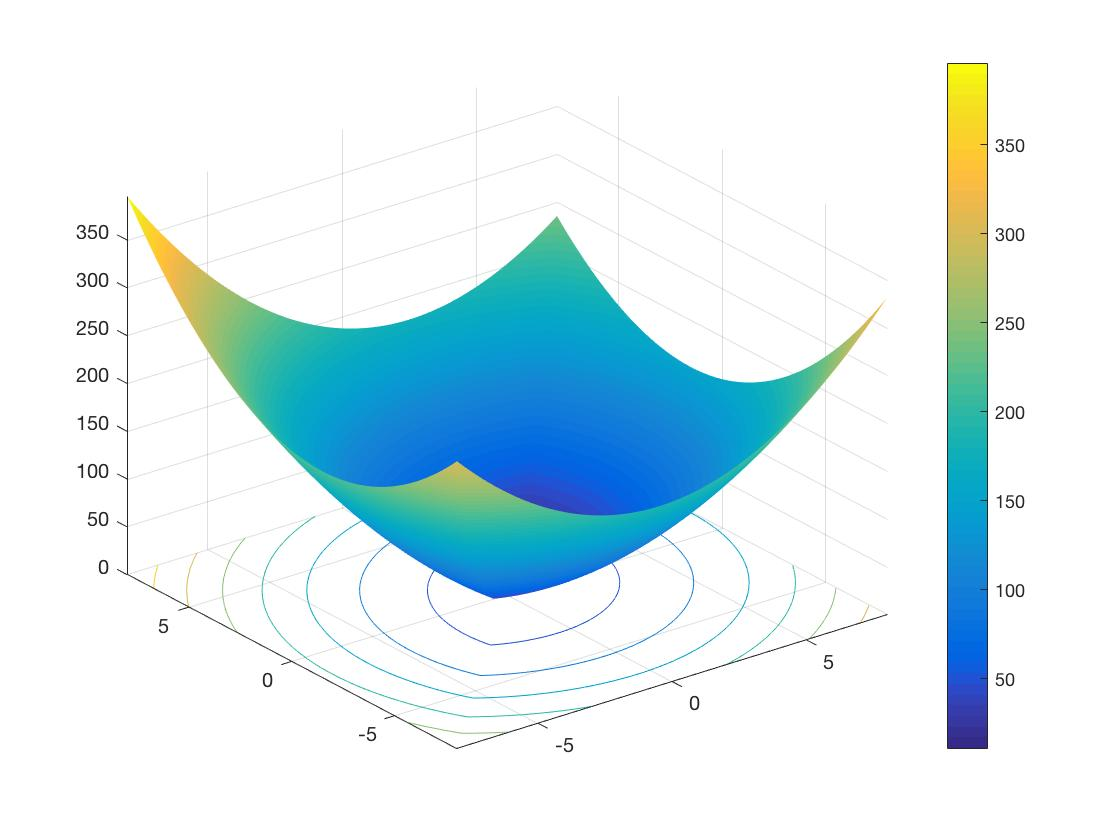
\includegraphics[width=2.2in]{q2c.jpg}
\caption{The 3D image for the function L}
\label{fig:q2c}
\end{minipage}
\end{figure}

\subsubsection{c}
\label{subsubsec:2.c}
In this case, the regularization parameter should be large enough according to Section \ref{subsubsection: 2.a}. 
After several times of test, $\lambda$ is kept $6$, which is large enough to obtain the optimal solution. And the optimal solution 
$$(m_-, m_+) = (0.5, 0.5)$$.

The code for plotting figures and calculating mean values is in Appendix \ref{app:b}.

\section{Some Programming \& Some Experimenting}

\subsection{Question 3}
\subsubsection{a}
In this case, I use gradient descent to find the mean values.
Since this is a two-class digit classification task in 64 dimensions, $L$ can be regard as a function of 128 variables. 
\begin{itemize}
\item Step 1: I assign these variables into two 64-digit-length vectors $m_-$ and $m_+$ with a random start point. 
\item Step 2: Then I calculate the loss function with the initial mean, the gradient of all the mean. And update the mean to the opposite direction if their gradient with certain learning rate. 
Then I calculate the new loss with updated mean and compare the difference between the two loss values.
\item Step 3: Loop in Step 2 until the difference is smaller than a certain termination error.
\end{itemize}
At last, the expected mean can be obtained. During this process, the learning rate and the $\lambda$ should be adjusted. 
When $\lambda$ is 0, the mean obtained does not change with the adjustment of learning rate. 
When $\lambda$ is very large, the first part of loss function can be ignored. 
Thus it becomes $$L = \lambda||m_- - m_ +||_1$$ 
To obtain the minimum value, $m_-$ and $m_+$ are expected to be almost the same. 
Thus when adjusting the learning rate of a large $\lambda$, I need to consider whether $m_-$ and $m_+$ obtained are as expected. 
Otherwise, if the learning rate is too large or too small, wrong mean may be obtained.

The code to implement gradient descent is in Appendix \ref{app: c}.

\subsubsection{b}
The two solution mean images I find for $\lambda=0$ are shown in Figure \ref{fig:q3a} and Figure \ref{fig:q3b}.
The two solution mean images for a large $\lambda$ are shown in Figure \ref{fig:q3c} and Figure \ref{fig:q3d}.
Here we can tell from these two images that $m_-$ and $m_+$ is almost the same with a large $\lambda$, which is the result expected.
Since $\lambda$ is very large in this case, the learning rate should be proper to find the mean. 
Here the learning rate is 0.00000001. 
In addition, it is better to use a dynamic learning rate in this case to let the learning rate decrease in every round of calculation. 
Or to use the optimized learning rate $\alpha$ that satisfied $$h`(\alpha) = \frac{\partial L(m+\alpha*dm)} {\partial (m+\alpha*dm)} dm$$
Here $m$ is the mean, which is the variable of loss function $L$, and $dm$ is the derivative of $m$. 
Since with adjustment of learning rate and $\lambda$ by myself still can find the expected result of mean, I do not use this method to control learning rate in every round.

\begin{figure}[!ht]
\begin{minipage}[t]{0.5\linewidth}
\centering

\includegraphics[width=2.2in]{q3a.jpg}
\caption{Image for $m_-$ with $\lambda = 0$}
\label{fig:q3a}
\end{minipage}%
\begin{minipage}[t]{0.5\linewidth}
\centering

\includegraphics[width=2.2in]{q3b.jpg}
\caption{Image for $m_+$ with $\lambda = 0$}
\label{fig:q3b}
\end{minipage}
\end{figure}

\begin{figure}[!ht]
\begin{minipage}[t]{0.5\linewidth}
\centering

\includegraphics[width=2.2in]{q3c.jpg}
\caption{Image for $m_-$ with a large $\lambda = 1250000 $}
\label{fig:q3c}
\end{minipage}%
\begin{minipage}[t]{0.5\linewidth}
\centering

\includegraphics[width=2.2in]{q3d.jpg}
\caption{Image for $m_+$ with a large $\lambda =1250000$}
\label{fig:q3d}
\end{minipage}
\end{figure}

\clearpage
\appendix
\section{Code for Question 1}
\label{app: a}
\begin{lstlisting}
% Question 1 (a)
m = -4:0.01:4; % range of m+
l0 = (-1-m).^2 + (1-m).^2 + 0*abs(1-m); % loss function with lambda 0
% plot all the loss function with lambda {0,2,4,6}
figure
plot(m,l0)
title('Loss function as a function of m+')
xlabel('m+')
ylabel('loss')
% Question 1 (b)
% the minimizer and the minimum values
m0 = min(l0);
m0_er = m(find(l0==m0));
% the point where the derivative equals 0
dx = 1e-3;
xi = -4:dx:4;
yi0 = interp1(m, l0, xi);
dyi0 = [0 diff(yi0)]/dx;
dy0 = interp1(xi, dyi0, m);
min_dy0 = min(abs(dy0(2:801)));
der0_pos1 = find(dy0==min_dy0);
m(der0_pos1)
l0(der0_pos1)
\end{lstlisting}

\section{Code for Question 2}
\label{app:b}
\begin{lstlisting}
%Question 2
m_minus = -8:0.01:8;
m_plus = -8:0.01:8;
[X,Y] = meshgrid(m_minus, m_plus);
L = (-1-Y).^2 + (1-Y).^2 + (3-X).^2 + (-1-X).^2 + 6*abs(X-Y);
% contour figure
figure
contourf(X,Y,L,20)
colorbar
% 3D figure
figure
surfc(X,Y,L)
colorbar
shading interp
% mean values
m = min(min(L));
[x,y] = find(L==m);
m_minus(x)
m_plus(y)
\end{lstlisting}

\clearpage

\section{Code for Question 3}
\label{app: c}
\begin{lstlisting}
M_m = zeros(1,size(X,2)); % initial values of m-
M_p = zeros(1,size(X,2)); % initial values of m+
lambda = 1250000;
m = 0.00000001; % learning rate
change = 1; % initial change
k = 0; % loop number
while min(abs(change)) > 0.00000001
    L = sum((X(1:554,:)-repmat(M_m,554,1)).^2) + sum((X(555:1125,:)...
    -repmat(M_p,571,1)).^2) + lambda*abs(M_m-M_p);
    dm = 554*2*M_m - sum(2*X(1:554,:))+lambda*sign(M_m-M_p); % gradient of m-
    dp = 571*2*M_p - sum(2*X(555:1125,:))-lambda*sign(M_m-M_p); % gradient of m+
    M_m = M_m - m * dm; % update m- to the opposite direction of its gradient
    M_p = M_p - m * dp; % update m+ to the opposite direction of its gradient
    L_temp = sum((X(1:554,:)-repmat(M_m,554,1)).^2) + sum((X(555:1125,:)...
    -repmat(M_p,571,1)).^2) + lambda*abs(M_m-M_p);
    change = L - L_temp;
    k = k + 1;
end

img01 = reshape(M_m,[8, 8]);
img1 = mat2gray(img01);
figure
imshow(img1, 'InitialMagnification', 'fit');
 
img02 = reshape(M_p,[8, 8]);
img2 = mat2gray(img02);
figure
imshow(img2, 'InitialMagnification', 'fit');
\end{lstlisting}



\end{document}